\documentclass[info]{ensrennesbeamer}

%\usepackage[T1]{fontenc}
\usepackage[utf8]{inputenc}
\usepackage[french]{babel}


\usepackage{listings}%

\usepackage[framemethod=tikz]{mdframed}
\usepackage{minted}
\usepackage{datetime}
\usepackage{xcolor}
\usepackage{graphicx}

\setminted{fontsize=\scriptsize,baselinestretch=1}

\tikzstyle{startstop} = [rectangle, rounded corners, minimum width=3cm, minimum height=0.5cm,
						text centered, draw=black, fill=red!30]
\tikzstyle{process} = [rectangle, minimum width=3cm, minimum height=0.5cm, text centered,
					   draw=black]
\tikzstyle{arrow} = [thick,->,>=stealth]
\author{J. Cabrita\and C. Legrand-Lixon\and A. Lequen\and G. Mescoff}
\title{Prog2 - Projet 1 \\ Interprète LISP}
%\setbeamercovered{transparent} 
%\setbeamertemplate{navigation symbols}{} 
%\logo{} 
\institute[]{ENS Rennes} 
\date{28 février 2018} 
%\subject{} 

\sloppy

\begin{document}

{
\setbeamerfont{frametitle}{size=\Huge}
\begin{frame}[plain]
\titlepage
\end{frame}
}

\section*{Introduction}
\begin{frame}
\textbf{Interprète LISP}
	\begin{itemize}
		\item LISP (1958) : langage de programmation fonctionnel
		\item Interprète : programme exécutant dynamiquement un script non compilé	
	\end{itemize}
\end{frame}

\begin{frame}
\tableofcontents
\end{frame}

\section{Interprète LISP}
\begin{frame}
\centering
	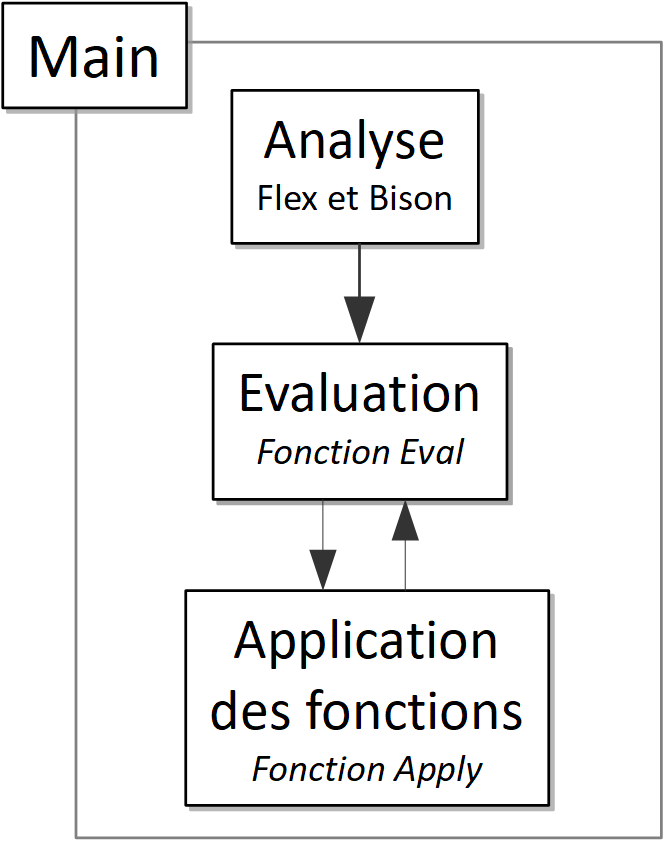
\includegraphics[height=0.8\textheight]{schema_fonctionnement.png}
\end{frame}

\subsection{Analyse}
\begin{frame}
\frametitle{Grammaire}
	\begin{block}{Forme de Backaus-Naur}
		\emph{expression} $\rightarrow$ \emph{list} $\vert$ \emph{number} $\vert$ \emph{symbol} $\vert$ \emph{string} $\vert$ \emph{nil} \\
		\emph{list} $\rightarrow$ \emph{(} \emph{expression} \emph{)}
	\end{block}
	$\rightarrow$ Lisp peut être décrit par des règles simples
\end{frame}

\begin{frame}{Analyses lexicale et syntaxique}

\begin{block}{\textbf{Flex} : Analyse lexicale}
	Transforme des chaînes reconnues par des expressions régulières en \emph{tokens}
\end{block}

\begin{block}{\textbf{Bison} : Analyse syntaxique}
	Convertit une suite de \emph{tokens} en objets reconnus par l'interprète
\end{block}
\end{frame}

\subsection{Environnement}
\begin{frame}{Principe}
	
	\textbf{Première approche : liaisons dynamiques}
	\begin{itemize}
	\item Structure de pile
	\item Liaisons jamais modifiées
	\item Liaisons masquées
	\end{itemize}
	
	\centering
	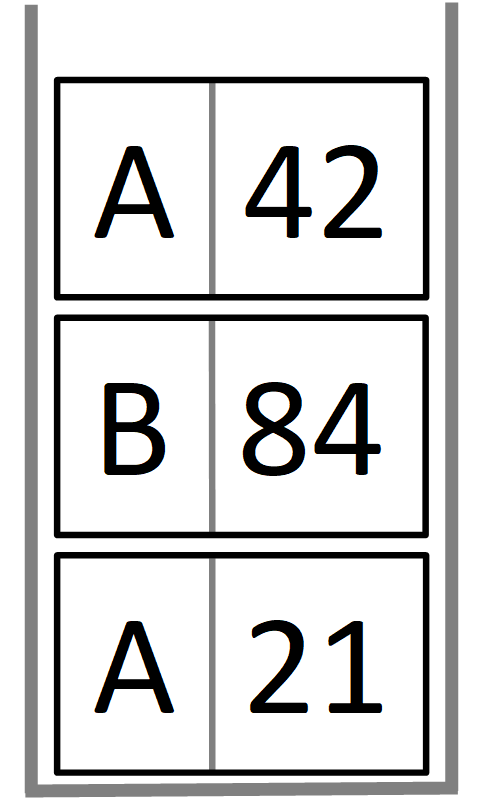
\includegraphics[height=0.6\textheight]{environnement_principe.png}
\end{frame}

\begin{frame}{Implémentation}
	\begin{block}{Liste chaînée}
		\begin{itemize}
			\item Facile à implémenter
			\item Recherche d'un élément assez longue		
		\end{itemize}
	\end{block}
	\centering
	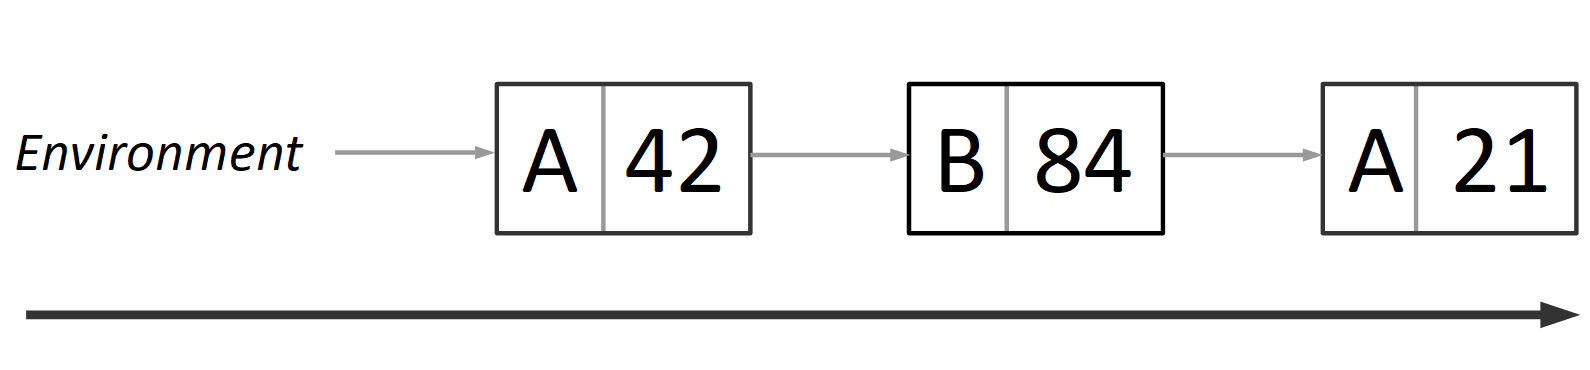
\includegraphics[width=1.0\textwidth]{environnement_implementation.png}
	
	\textbf{Idée} : remplacer par une table de hachage
\end{frame}

\subsection{Dynamisme}
\subsubsection{Évaluation des expressions}
\begin{frame}
	\begin{block}{Fonction \lstinline[][eval[}
		Renvoie la valeur de l'expression passée
		\begin{itemize}
			\item Chercher les valeurs des symboles dans l'environnement
			\item Modifier l'environnement
			\item Identifier les sous-routines natives
			\item \textbf{Demander l'application des sous-routines}
		\end{itemize}
	\end{block}
	\begin{alertblock}{Gestion des erreurs}
		Lève une exception en cas d'incohérence sémantique
	\end{alertblock}

\end{frame}

\subsubsection{Applications des mots-clés}
\begin{frame}
	\begin{block}{Fonction \lstinline[][apply[}
		Applique une fonction à une liste d'arguments
		\begin{itemize}
			\item Vérifie si la liste commence par une fonction
			\item Applique la fonction aux arguments passés
			\item Retourne la valeur de l'expression évaluée
		\end{itemize}
	\end{block}

\end{frame}

\begin{frame}	
	\begin{exampleblock}{Remarques : Fonction \lstinline[][apply[}
		\begin{itemize}
			\item Mutuellement récursive avec \lstinline[][eval[
			\item Ignore les arguments supplémentaires
		\end{itemize}
	\end{exampleblock}
	
	\begin{alertblock}{Gestion des erreurs}
		Lève une exception si :
		\begin{itemize}
			\item Le premier élément n'est pas évalué en une fonction
			\item Trop peu d'arguments suivent
		\end{itemize}
	\end{alertblock}
	
\end{frame}

\begin{frame}
	\begin{block}{Implémentation des différentes sous-routines }
		\begin{itemize}
			\item Sous-routines implémentées dans des fonctions propres
			\item Conventions de nommage et de prototypes
		\end{itemize}
		\textbf{Ajout rapide de nouvelles fonctions natives}
	\end{block}

	\begin{exampleblock}{Exemples de sous-routines natives}
		\begin{itemize}
			\item \lstinline[][+[, \lstinline[][*[, \lstinline[][-[, ...
			\item \lstinline[][lambda[, \lstinline[][quote[, \lstinline[][print[, \lstinline[][setq[, \lstinline[][newline[...
			\item \lstinline[][apply[, \lstinline[][eval[
			\item \lstinline[][progn[, \lstinline[][map[
			\item \lstinline[][printenv[
		\end{itemize}
	\end{exampleblock}
\end{frame}

\section{Vers un interprète à liaison statique}
\subsection{Liaisons statiques}

\begin{frame}
	\textbf{Deux manières de modifier les liaisons}
		\begin{block}{Dynamique : \lstinline[][define[}
			\begin{itemize}
				\item Ajoute une nouvelle liaison à la liste
				\item Masque les liaisons précédentes
			\end{itemize}			
		\end{block}
	\centering
	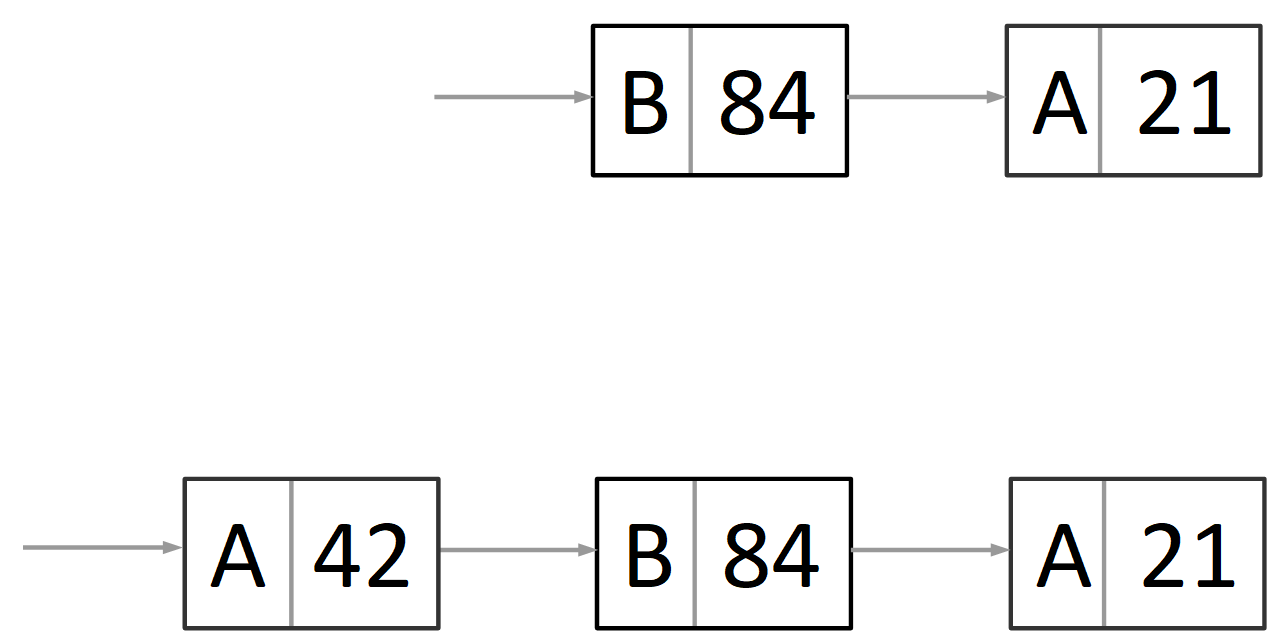
\includegraphics[height=0.5\textheight]{liaisons_statiques.png}
	
\end{frame}

\begin{frame}
	\textbf{Deux manières de modifier les liaisons}
		\begin{block}{Statique : \lstinline[][setq[}
			\begin{itemize}
				\item Crée une nouvelle liaison si le symbole n'est pas encore lié
				\item Modifie la liaison la plus récente pour un symbole dans l'environnement courant
			\end{itemize}
		\end{block}
	\centering
	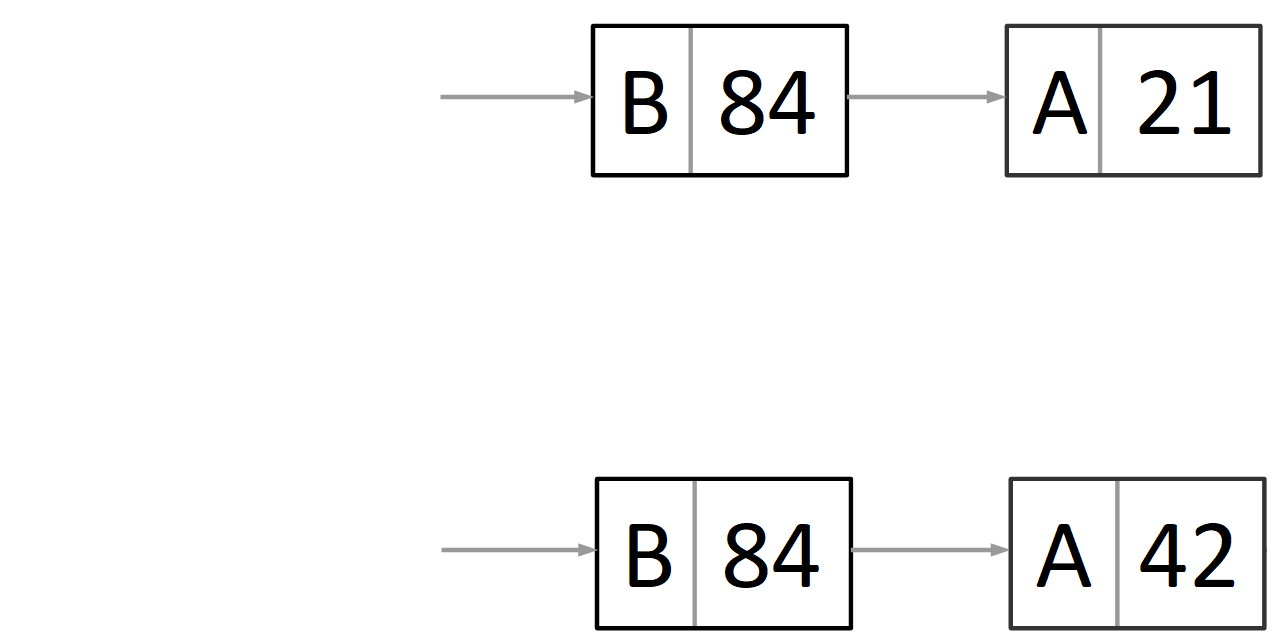
\includegraphics[height=0.5\textheight]{liaisons_dynamiques.png}
		
\end{frame}


\subsection{Clôtures}
\begin{frame}
	\begin{block}{\emph{Closure}}
		Capture (\emph{snapshot}) de l'environnement au moment de la déclaration d'une lambda-expression
	\end{block}
	\begin{block}{Implémentation}
		\begin{itemize}
			\item Enregistre l'environnement à chaque symbole \emph{lambda}.
			\item Pointeur vers un environnement
		\end{itemize}
	\end{block}
	
\end{frame}

\section{Conclusion}
\subsection{Conclusion}
\begin{frame}
	\begin{block}{Conclusion}
		\begin{itemize}
		\item Interprète à liaison dynamique et statique robuste
		\item Meilleure compréhension des mécanismes
		\item Nombreuses pistes pour poursuivre
		\end{itemize}
	\end{block}
\end{frame}

\subsection{SWOT}
\begin{frame}
	\begin{block}{SWOT}
		\begin{itemize}
			\item \textbf{Forces :} Organisation agile, planification
			\item \textbf{Faiblesses :} Gestion hasardeuse des tests et exceptions
			\item \textbf{Opportunités :} Meilleure compréhension de la gestion de l'environnement. Mise en place méthode agile
			\item \textbf{Menaces :} Importance de l'organisation, de la robustesse du code et des tests
		\end{itemize}
	\end{block}
\end{frame}

\end{document}